\documentclass[12pt]{article}
\usepackage{amsmath}
\usepackage{csvsimple}
\usepackage{graphicx}
\graphicspath{ {./../images/} }
\usepackage{hyperref}
\usepackage[latin1]{inputenc}
\usepackage{listings}
\usepackage{algorithm2e}
\SetKwComment{Comment}{/* }{ */}

\DeclareMathOperator{\Tr}{Tr}

\lstset{
  columns=fullflexible,
  breaklines=true,
}

\title{El Farol Bar Problem on a Social Network}
\author{Rebecca Cohen}

\begin{document}
\maketitle
\section{Abstract}
The El Farol Bar problem is a classic game theory model in which independent agents learn to use a heterogeous distribution of strategies to share a limited resource while avoiding congestion.  This paper analyzes what happens if instead of choosing whether to attend the bar or not independently, agents attempt to attend the bar with their friends on a social network.  We find that depending on the combination of threshold and network structure, agents may develop a heterogeneous distribution of behaviors that can utilize the resource without overcrowding it.  We derive an algorithm to identify the largest possible fixed point on a given network, but show that this fixed point is often unreachable.  Using numerical algorithms, we test the impact of edge density, heterogeneity of degree, community structure, and random noise, finding that noise, as well as edge density can contribute to higher attendance rates, heterogeneous degree distributions lead to less sensitivity to initial conditions, and community structure leads to an increased variability of outcome and increased frequency of period 2 limit cycles.  Wholistically, these results show that agents following the same strategy in different network contexts can behave similarly to those following different strategies independently.

\section{Introduction}

The El Farol Bar problem, named and popularized by Brian Arthur, is a stylized model in which agents attempt to utilize a limited resource while avoiding congestion \cite{arthur:1994}.  The name of the problem is inspired by a bar called El Farol in Santa Fe, which had a popular weekly event with live music.  Everyone enjoys the evening if the space is not overcrowded, but if too many people attend, everyone will have a worse time than if they had stayed home.

In Arthur's original publication, each agent has access to a finite pool of fixed strategies, as well as weekly attendance history for the entire system.  At each timestep, the agent selects the strategy that would have led to the best performance over some recent time window.  In the original setup and many later variants, weekly attendance will never completely stabilize but will oscillate around the congestion threshold \cite{arthur:1994} \cite{chen:2012} \cite{zambrano:2004}.  While attendance is attracted to a certain range, the distribution of strategies amongst agents may not stabilize, although given a set of just two or three initial strategies, the system may converge to a stable and predictable attractor depending on the initial strategy distribution \cite{stLuce:2020}.

Scholars have motivated the importance of this problem with applications such as traffic and public transit congestion, internet traffic, and financial markets \cite{zambrano:2004} \cite{chen:2012}.  In these applications, modeling agents as behaving independently and attempting to optimize solely their own utility may be a reasonable model for empirical behaviors.  However, humans are social animals and in many situations, including the original story motivating the El Farol bar problem, agents may not only prefer to avoid crowding, but also prefer the company of friends.  Thus agents must balance two competing priorities, local conformity and global non-comformity.  In addition to attendance at bars, modeling this scenario could represent many other social behaviors such as trends in fashion and music.

There are variants of the El Farol problem that use coordination between agents to allow agents a broader choice of optimal strategies, although in such cases group coordination leads to lower overall utility as groups sharing the same strategy drive overcrowding. \cite{collins:2017} \cite{wilensky:2015}.  In addition, a variant of the problem has agents in a social network where agents' choices to go to the bar depend on their neighbors' history.   When these simulations are run on very regular network structures, a range of diverse equilibria can occur \cite{chen:2012}.  However, the agents have no innate preference to attend with or without their neighbors.

To model agents with a preference to attend the bar together, we construct a model in which each agent chooses whether to attend at time $t = 1$ based on their neighbor's behaviors at time $t$.  The strategy that can be varied then is the threshold value for attendance.  Without adaptive learning, this model resembles the threshold model for binary opions, which has been rediscovered and published in different contexts by economist Thomas Schelling \cite{schelling:1978} and sociologist Mark Granovetter \cite{granovetter:1978} \cite{grabish:2020}.  

If agents' thresholds are sufficiently low relative to their degrees on a fixed network, then the action, in this case attending the bar, would spread over the entire network, leading to congestion.  However, if the thresholds are too high, no agent will ever attend.  Between these two extremes, threshold models may have many stable or semi-stable fixed points \cite{adam:2012} and hysteresis \cite{Wiedermann_2020}.  Threshold models may also have limit cycles.  On an undirected network, these can be shown to always have period 2 \cite{grabish:2020} \cite{goles:1980}.

In the context of the El Farol bar problem, this paper will explore the impact of network structure on the dynamics of this intermediate regime.  When will network structure lead to suitably varied limiting behavior such that the bar can maintain attendance by a group of regulars without becoming overcrowded?  

We consider the impact of mean degree, heterogeneity of degree, and community structure on the number of agents attending, the sensitivity of the system to initial conditions, and the frequency of period 2 limit cycles.  We also consider the impact of random noise and examine the stability of fixed points on a particularly regular network.

\section{Model Specification}
To test the hypothesis that local differences in the structure of social networks can encode the diversity of strategies required to regulate attendance, we construct a simple scenario in which each agent chooses to attend the bar if at least $\ell$ of the agent's neighbors attended the previous week.  We define the attendance vector $\vec{y}(t)$ such that
\begin{equation}
  y_i(t) = \begin{cases}
    1 &\text{if agent}\; i \; \text{attends on week t} \\
    0 &\text{otherwise}
  \end{cases}
\end{equation}

Then 
\begin{equation}
  \vec{y}(t + 1) = F(\mathbf{A}\vec{y}(t))
\end{equation}

where
\begin{equation}
  F(\vec{x})_i = \begin{cases}
    1 &\text{if} \; x_i \geq \ell \\
    0 &\text{otherwise}
  \end{cases}
\end{equation}

A traditional implementation of the El Farol bar problem would require some mechanism for modulating attendance patterns depending on the congestion level at the bar.  However, this paper will focus on the regulatory effect of the network structure itself.  As we shall see, in many cases the interaction of network structure with an appropriate choice of $\ell$ will maintain attendance below the traditional 60\% threshold. 

\section{Fixed Points}

Fixed points of this system occur where

\begin{equation}
  \vec{y}_{\infty} = F(\mathbf{A}\vec{y}_{\infty})
\end{equation}

Unsurpisingly, the trivial fixed point of $\vec{y}_{\infty} = \vec{0}$ is a solution since $\mathbf{A}\vec{0} = \vec{0}$ and $F(\vec{0}) = \vec{0}$.  There may also be nontrivial fixed points, depending on the network and $\ell$.  Let $S$ denote a subset of nodes such that every element of $S$ has at least $\ell$ neighbors in $S$ and no element of $S^C$ has $\ell$ neighbors in $S$.  If we construct $\vec{y}$ such that  
\begin{equation}
  y_i = \begin{cases}
    1 &\text{if} \; i \in S \\
    0 &\text{otherwise}
  \end{cases}
\end{equation}
 then for all $i \in S$, $\mathbf{A}\vec{y} \geq \ell$ and for all $y \notin S$, $\mathbf{A}\vec{y} < \ell$.  Thus $\vec{y} = \mathbf{A}\vec{y}$. 

In general, we cannot expect $S$ to be unique.  As a simple example, suppose the network contains two mutually exclusive $\ell$-cliques, each of which is connected to the rest of the network by less than $\ell$ edges.  Then the network must have at least 3 nontrivial fixed points, consisting of the vertices in one or both cliques.

Algorithm 1 finds a fixed point of an arbitrary graph $G=(V,E)$.  We show that it will return the maximally large fixed point (MFP) possible, and that the MFP is unique for any $G$.

\begin{algorithm}
  \caption{Find MFP}\label{alg:two}
  \KwData{$G = (V, E)$, $\ell$}
  $G'(V', E') \gets G(V, E)$; \\
  $N \gets 0$; \\
  \While{$V'.size \neq N$}{
    $N \gets $ V'.size\;
    Delete all vertices with degree $< \ell$ \\
    Remove all dangling edges
  }
  \Return{V'}
  \end{algorithm}

  The termination condition of the while loop guarantees that every element of $V'$ has at least $\ell$ neighbors in $V'$.  Therefore, $V'$ must be a fixed point of $G$ with respect to $\ell$.  
  
  To show that $V'$ is the unique MFP, we introduce the following invariant that must be true at every iteration of the while loop: any $v \in V$ such that $v \notin V'$ cannot be in a fixed point of $G$ with respect to $\ell$.

  On initialization, all elements of $V$ are in $V'$ so the invariant is trivially true.  During execution, the loop invariant guarantees that all possible elements of a fixed point are in $V'$, so any elements that are deleted cannot have $\ell$ neighbors in the fixed point.  Therefore they cannot be in the fixed point themselves.  On exit, no additional nodes are deleted from $V'$.  So any node $v \notin V'$ cannot be a part of a fixed point and $V'$ contains the maximum possible set of nodes whose attendance could be a fixed point with respect to $\ell$. 

\section{Numerical Simulations}
We can use numerical simulations to gain a stronger understanding of the steady state behavior of the system.  We use three different random graph models: the Erdos-Renyi random graph, in which all possible edges exist with equal probability, the Chung-Lu model, which weights edge probabilitiies to obtain a target degree distribution, and the stochastic block model (SBM), in which the probabiliity of an edge is depends on its membership in a particular block.  Comparing the results on the Erdos-Renyi network vs. the Chung-Lu model, generated with a power law degree distribution, allows us to evaluate the impact of a heterogeneous degree distribution on the steady state of the system, while the SBM allows us to explore the impact of community structure.

\subsection{Mean Degree}
Figure 1 shows the weekly attendance on each of the three random graph models.  Both the Erdos-Renyi model and the SBM have close to zero attendance when the mean degree is under 10, and universal attendance when the mean degree is above 13.  In between, weekly attendance grows abruptly, but there is high variance with many trials still having no limiting attendance well above what appears to be the critical threshold.

In contrast, as degree increases on the Chung Lu model, attendance grows much more slowly over a larger range of values.  Most of the random networks generated produce identical or close to identical results between trials.

The remainder of this paper will focus on the intermediate region in which some but not all agents attend at steady state.  While we cannot generate random networks with identical degree, we use a target range of $\langle k \rangle \in [10, 11]$ to generate roughly comparable networks in this region.

\begin{figure}
  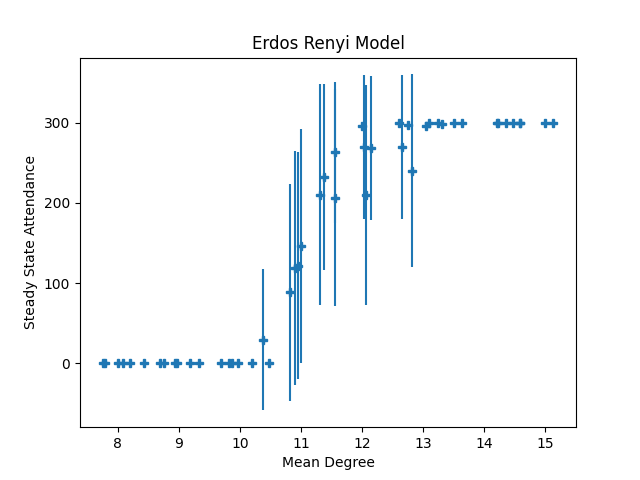
\includegraphics[width=0.32\textwidth]{erdos_renyi_degree.png}
  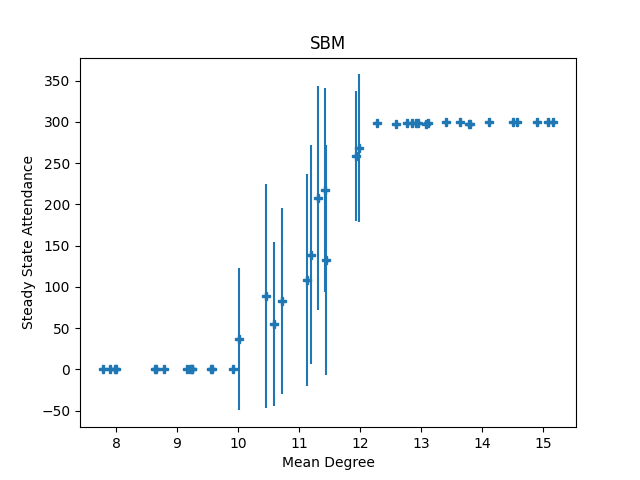
\includegraphics[width=0.32\textwidth]{sbm_degree.png}
  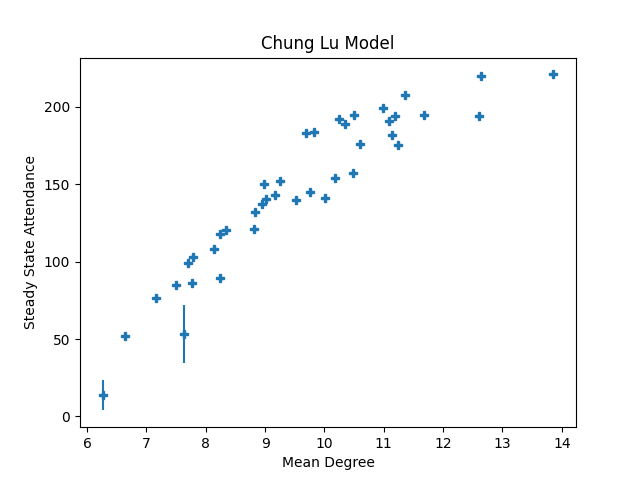
\includegraphics[width=0.32\textwidth]{chung_lu_degree.png}
  \caption{Weekly attendance patterns on random networks with varying mean degree.  $\ell = 4$}
\end{figure}

\subsection{Variability of Outcomes}
\begin{figure}[h!]
  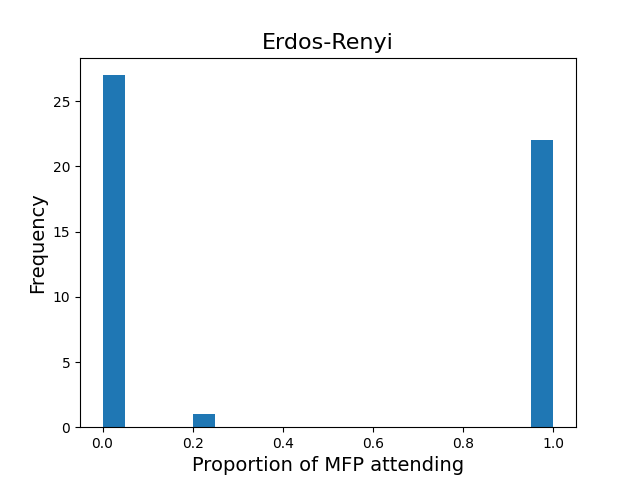
\includegraphics[width=0.32\textwidth]{gnp_attendance.png}
  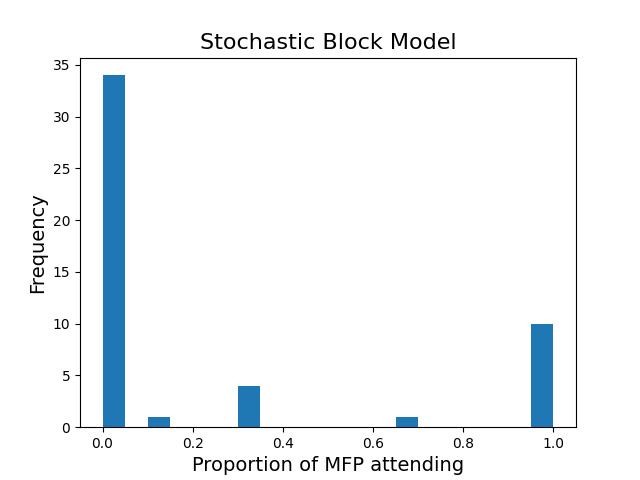
\includegraphics[width=0.32\textwidth]{sbm_attendance.png}
  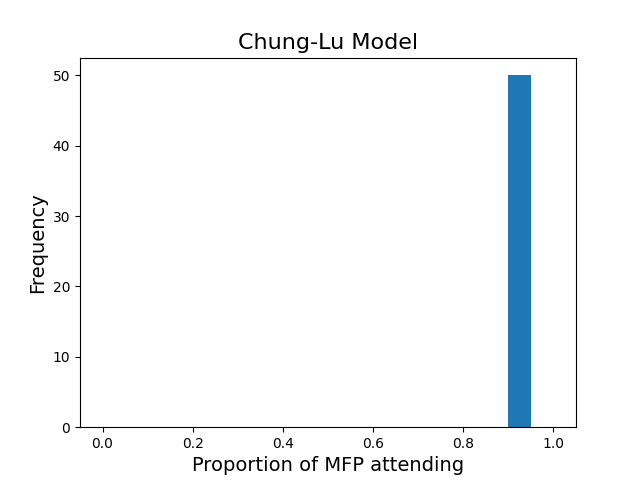
\includegraphics[width=0.32\textwidth]{cm_attendance.png}
  \caption{Weekly attendance pattern on fixed random networks across multiple trials}
\end{figure}

Figure 2 shows weekly attendance numbers on these random graphs over repeated trials with varying initial conditions.  Attendance converges to a consistent count in most but not all trials.  However, even on the same network with the same number of agents attending at $t=0$, weekly attendance varies between trials.  In both the Erdos-Renyi and SBM simulations, some initial conditions (wiith 30\% of agents attending) led to no agents attending at steady state, while others led to attainment of the maximal fixed point.  In addition, there were intermediate states in which a fraction of the MFP attended while other members of the MFP never attended.  These intermediate states were much more frequent on the SBM versus the Erdos-Renyi model. 

In contrast, the Chung-Lu model leads to much more stable results.  However, results are still not identical between trials, and no trial attained the MFP.  To further test the relationship between heterogeneous degree distribution and variations in steady state attendance, figure 3 (left) plots the standard deviation of the degree distribution against the standard deviation of steady state attendance between multiple trials on fixed networks.  Mean degree was held steady between trials.  This experiment validates the observation that more varied degree sequences lead to more stable attendance patterns, although the plot also highlights the role of randomness in determining whether a network will have multiple reachable steady states.

\begin{figure}
  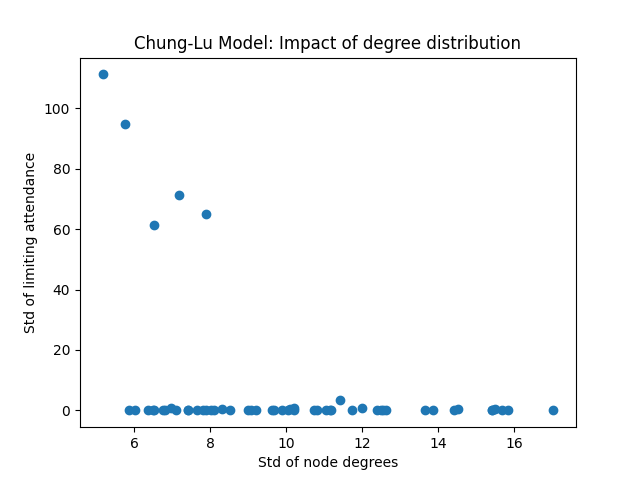
\includegraphics[width=0.45\textwidth]{chung_lu_std.png}
  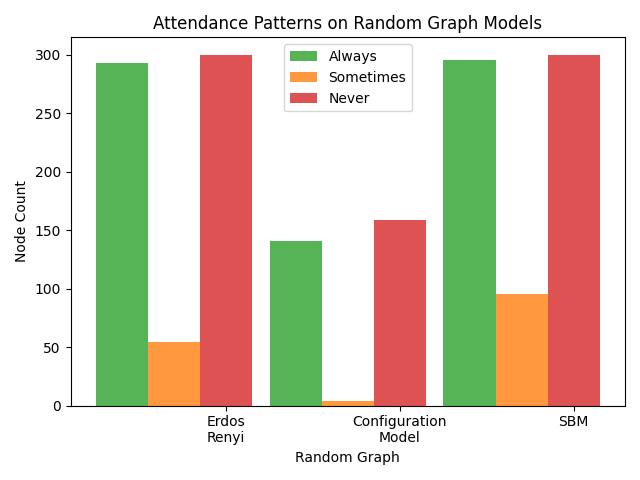
\includegraphics[width=0.45\textwidth]{always_sometimes_never.png}
  \caption{Standard deviation of degree distribution vs. steady state attendance patterns on the Chung-Lu model (left).  Fraction of agents observed attending always, sometimes, or never in at least one trial (right).}
\end{figure}

All three models had some trials with limit cycles of period 2.   These limit cycles are the result of coupled agents that reach the threshold dependent on each other's behavior.  If one agent but not the other attends as part of the initial conditions, the two agents will toggle back and forth indefinitely, caught in a game of telephone tag in which they miss running into each other at every timestep.  In some cases, more complex interactions occur, involving more than two agents.

Figure 3 (right) shows the number of distinct agents attending always, sometimes, or never in at least one trial for each of the three random graph models.  The figure shows the contrast between the Chung-Lu model with a heavy-tailed degree distribution, which has around half of the nodes in the Always and Never camp, and very few in Sometimes, compared with the Erdos-Renyi and stochastic block models, which have a much more variabiliity.  These results suggest that more homogeneous degree distributions increase the probability of agents engaging in telephone tag behaviors, as well as variability in steady state attendance.

Figure 4 shows the extreme case where nodes are arranged in a 2-dimensional lattice with edges wrapping around at the boundaries, once again with $\ell = 4$.  In this case, universal attendance is a fixed point, but even a single agent failing to attend will trigger telephone tag, beginning at the epicenter of the disruption and spreading across the entire network.  When an agent fails to attend in the telephone tag scenario, nonattendance spreads across the network.  This extreme example may build intuition about the observed phenomenon that more homogeneous degree distributions have higher rates of telephone tag.   

\begin{figure}[h!]
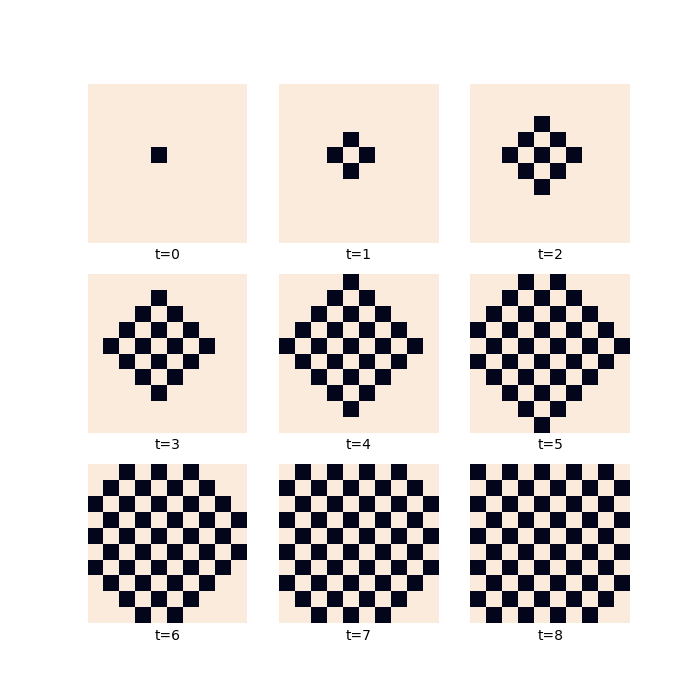
\includegraphics[width=0.5\textwidth]{one_minus.png}
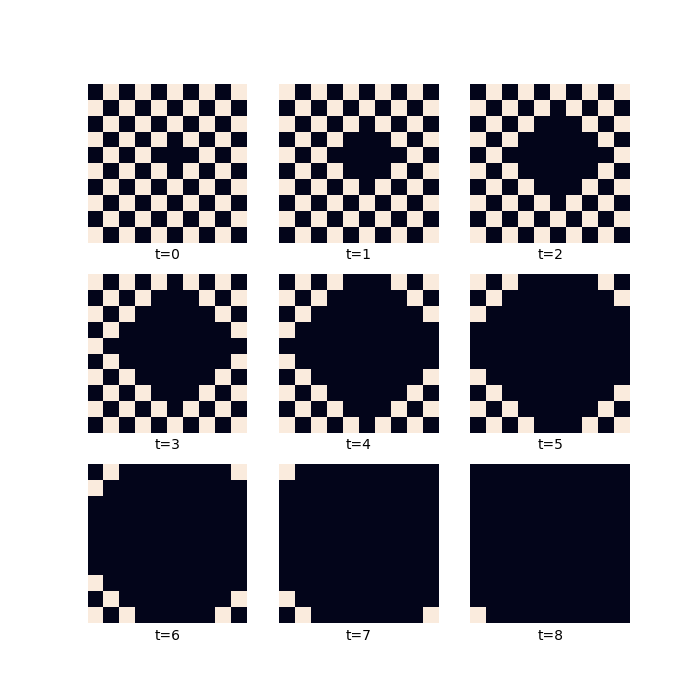
\includegraphics[width=0.5\textwidth]{alt_minus.png}
\caption{Unstability with respect to negative perturbations of universal attendance (left) and universal telephone tag (right) on a 2-dimensional lattice.}
\end{figure}

\subsection{Random Noise}

When each node has degree exactly $\ell$, we have seen that the presence of randomness drives attendance down.  However, with sufficient density of edges, noise could allow otherwise unreachable nodes in the MFP to begin attending.  To test the impact of noise on random networks, we introduce a new parameter, $\epsilon$ to govern the noisiness of the system.  We define

\begin{equation}
  F'(\vec{x})_i = \begin{cases}
    1 - F(x_i) &\text{with} \\
    & \text{probabiliity} \epsilon \\
    F(x_i) &\text{otherwise}
  \end{cases}
\end{equation}

and set
\begin{equation}
  \vec{y}(t + 1) = F'(\mathbf{A}\vec{y}(t))
\end{equation}

\begin{figure}
  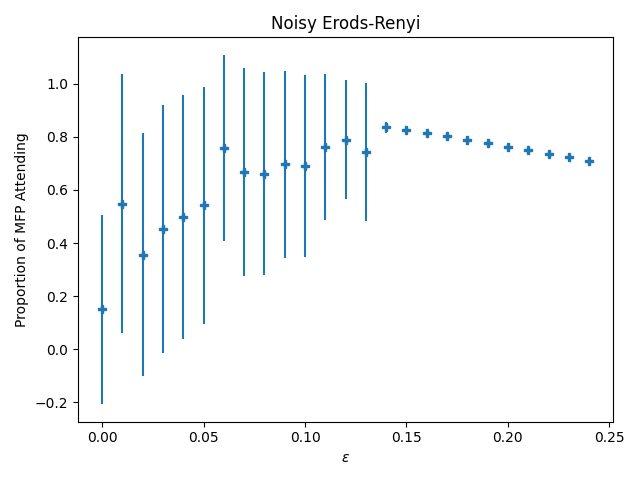
\includegraphics[width=0.32\textwidth]{noisy_erdos_renyi.png}
  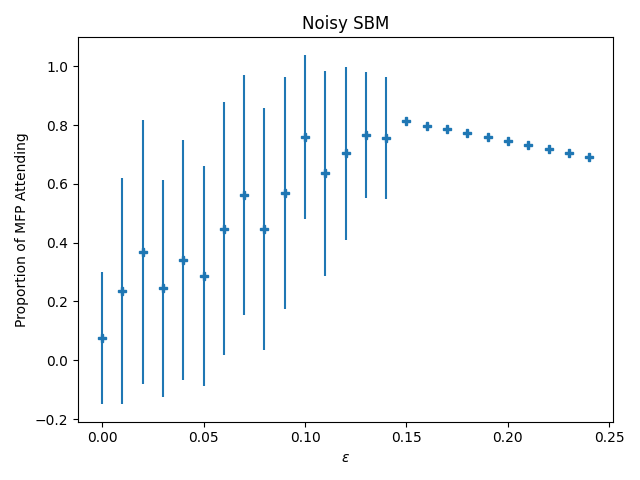
\includegraphics[width=0.32\textwidth]{noisy_sbm.png}
  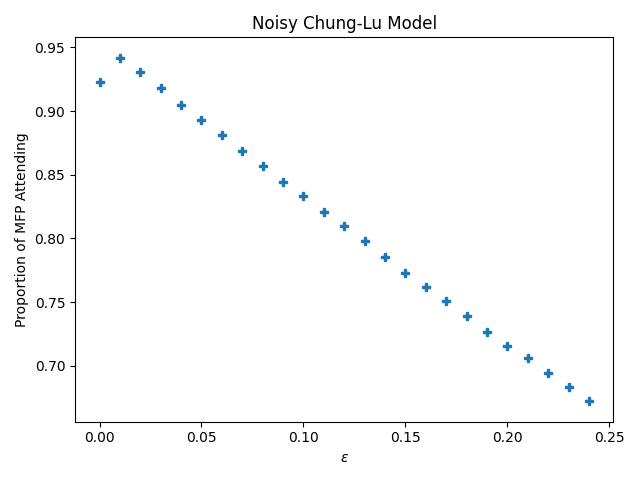
\includegraphics[width=0.32\textwidth]{noisy_chung_lu.png}
  \caption{Impact of noise level $\epsilon$ on random graph models}
\end{figure}

Figure 5 shows the impact of $\epsilon$ on the same three random graph models from section 5.  As usual, the Chung-Lu model with power law degree distribution had little variability between trials, and attendance decreases as $\epsilon$ increases.  On the Erdos-Renyi and SBM experiments, which have homogeneous degree distributions, increasing $\epsilon$ from 0 to around 0.14 increases weekly attendance and decreases the standard deviation between trials.  To make sense of this behavior, we note that nodes in the MFP may come in smaller pockets that are less densely connected to the rest of the network.  Adding noise may allow some otherwise unreachable nodes to begin attendiing.  As $\epsilon$ continues to grow, there is an abrupt transition after which the standard deviation is close to 0 and attendance begins decreasing.  More work is needed to come to a deeper understanding of why the transition is so abrupt, but at higher $\epsilon$ levels, it appears that all elements of the MFP are reachable.  Those that have sufficient redundancy to withstand the noise attend in the steady state.  

\section{Discussion}

The El Farol Bar problem has traditionally considered a population of agents with diverse strategies attempting to share a limited resource.  Traditional strategies often result in some agents attending always, some attending never, and some attending periodically, with a total attendance close to the tolerance threshold\cite{arthur:1994} \cite{stLuce:2020}.

In this paper, we find that a population of agents all following the same network-based strategy can behave similarly to the system of agents with heterogeneous strategies, with a subset of agents always attending, a subset never attending, and a subset attending periodically.  Furthermore, we have see how the interaction of the threshold, network structure, and random noise can effect the strategy distribution, with higher mean degrees, and, in some regimes increased noise leading to higher rates of attendance, and heterogeneous degree distributions leading to decreased sensitivity to initial conditions and lower rates of telephone tag behaviors.

The observations in this paper could help us design a network that would exhibit various strategy distributions from the El Farol Bar problem, but a natural extension of this work would be to reintroduce the evolutionary or inductive learning component that characterizes previous work on the El Farol bar problem.  We could have agents vary their $\ell$ value based on past performance, or allow them to modify network structure, forming new edges if they do not have sufficient friends in attendance, or removing edges if they are encountering congestion.  It could also be interesting to examine the results of these processes on empirical social network datasets, which tend to be much less locally treelike than the random graph models examined.    

\bibliographystyle{plain} % We choose the "plain" reference style
\bibliography{refs} % Entries are in the refs.bib file
\section*{Code}

\subsection{Functions for running simulation}
\lstinputlisting[language=Python]{../scripts/simulation.py}

\subsection{Functions for generating Chung-Lu Model}
\lstinputlisting[language=Python]{../scripts/chung_lu.py}

\subsection{Figure 1}
\lstinputlisting[language=Python]{../scripts/degree.py}

\subsection{Figures 2 and 3 (right)}
\lstinputlisting[language=Python]{"../scripts/Always Sometime Never.py"}

\subsection{Figure 3 (left)}
\lstinputlisting[language=Python]{"../scripts/Chung Lu Degrees.py"}

\subsection{Figure 4}
\lstinputlisting[language=Python]{../scripts/VN.py}

\subsection{Figure 5}
\lstinputlisting[language=Python]{../scripts/noise.py}

\end{document}